\documentclass{article}
\usepackage{natbib}

% if you need to pass options to natbib, use, e.g.:
%     \PassOptionsToPackage{numbers, compress}{natbib}
% before loading neurips_2018

% ready for submission
% \usepackage{neurips_2018}

% to compile a preprint version, e.g., for submission to arXiv, add add the
% [preprint] option:
%     \usepackage[preprint]{neurips_2018}

% to compile a camera-ready version, add the [final] option, e.g.:
     \usepackage[final]{neurips_2018}

% to avoid loading the natbib package, add option nonatbib:
%     \usepackage[nonatbib]{neurips_2018}


\usepackage[utf8]{inputenc} % allow utf-8 input
\usepackage[T1]{fontenc}    % use 8-bit T1 fonts
\usepackage{hyperref}       % hyperlinks
\usepackage{url}            % simple URL typesetting
\usepackage{booktabs}       % professional-quality tables
\usepackage{amsfonts}       % blackboard math symbols
\usepackage{nicefrac}       % compact symbols for 1/2, etc.
\usepackage{microtype}      % microtypography
\usepackage{graphicx}

\graphicspath{{./images/}}


\title{Denoising face recognition via clustering techniques}

% The \author macro works with any number of authors. There are two commands
% used to separate the names and addresses of multiple authors: \And and \AND.
%
% Using \And between authors leaves it to LaTeX to determine where to break the
% lines. Using \AND forces a line break at that point. So, if LaTeX puts 3 of 4
% authors names on the first line, and the last on the second line, try using
% \AND instead of \And before the third author name.

\author{Trung Vu, Sihyun Lee, Alexandre Lamy%
  % David S.~Hippocampus\thanks{Use footnote for providing further information
  %   about author (webpage, alternative address)---\emph{not} for acknowledging
  %   funding agencies.} \\
  % Department of Computer Science\\
  % Cranberry-Lemon University\\
  % Pittsburgh, PA 15213 \\
  % \texttt{hippo@cs.cranberry-lemon.edu} \\
  % examples of more authors
  % \And
  % Coauthor \\
  % Affiliation \\
  % Address \\
  % \texttt{email} \\
  % \AND
  % Coauthor \\
  % Affiliation \\
  % Address \\
  % \texttt{email} \\
  % \And
  % Coauthor \\
  % Affiliation \\
  % Address \\
  % \texttt{email} \\
  % \And
  % Coauthor \\
  % Affiliation \\
  % Address \\
  % \texttt{email} \\
}

\begin{document}
% \nipsfinalcopy is no longer used

\maketitle

\begin{abstract}
  In this paper we address the problem of detecting and recognizing specific objects (such as the faces of a specific group of people)
  in real life videos. By using unsupervised clustering techniques, we are able to exploit the inter-frame relationships in the
  video to significantly improve the accuracy of basic object detection and recognition algorithms. This yields results which are
  also much more robust to frame switches, lengthy occlusions, and variable numbers of targeted objects leaving and reentering the frames
  (all common occurrences in real life videos) than standard tracking techniques.
\end{abstract}

\section{Introduction}
% setting
% problem statement
% overview of issues and our solution

% Alex


One of the most interesting and difficult problems in computer vision is that of recognizing and then tracking an
entity of interest over time (i.e. in videos). This can be useful for surveillance of suspect individuals,
analysis of video data (music videos, concerts, sports games, etc.), or in building robots that interact with their
environment.

While tracking is a topic that has been extensively studied (see \cite{benchmarksurvey}), it is usually
done so in isolation from recognition. To track the object of interest, the leading tracking algorithms mainly rely on
properties of videos, notably that tracking target(s)
will move by small amounts at a time. This allows the algorithms to detect/infer the object(s) positions from the previous ones by
focusing on the region around the previously known position. While, these methods can work remarkably well on a clean video, such techniques have
little hope when faced with long occlusions or frequent ``frame switches'' as these will cause a violation of the assumptions that the algorithms are based on.

Alternatively, object detection techniques could be applied frame by frame. This would result in a much more robust result since the algorithms
make no assumptions concerning the relations between different frames. Hence, occlusions and frame switches pose no issue whatsoever. Unfortunately, even
the best of these methods result in relatively noisy or inaccurate results when compared with the tracking algorithms. This can be attributed to the fact that the detection
algorithms make no use of the wealth of information provided by the inter frame relationships (notably that most objects will usually not move by a large distance).

In this paper we propose a novel post-processing method, based on unsupervised clustering techniques, to ``denoise'' results obtained
from object detection algorithms by exploiting inter-frame relationships. The result is a technique that is more robust to occlusions and frame switches than the standard
tracking techniques and more accurate (less noisy) than the results obtained by naively applying object detection algorithms. We also have the added benefit of being able to easily
do object recognition at the same time as detection. Our method will not only reduce the noise in the detection error (bad bounding boxes) but also in the classification error (bad labels).

\section{Standard tracking methods and issues}
% tracking really isn't robust for complicated videos (varying number of people, frame switches, etc.)

Our problem, that of detecting objects throughout a video, or variations of it are often solved via tracking techniques. As mentioned above, the core idea is to exploit
inter-frame relations, notably the assumption that most objects will not move by much between frames, to track or follow the various target objects. We quickly summarize
the main tracking algorithms used in practice and show that they rely on core assumptions which are violated
when faced with real life videos which contain frame switches, long occlusions, and various target objects coming in and out
of the frames in variable number. In the presence of these realities, we show that these tracking algorithms are unusable.

As mentioned in \cite{benchmarksurvey}, the most commonly used tracking algorithms are OLB \cite{OLB}, IVT \cite{IVT}, MIL \cite{miltrack}, L1 \cite{L1}, and TLD \cite{TLD}.
We give a quick summary of each and outline their main issue in our context.

OLB or tracking via on-line boosting is a tracking method described in \cite{OLB} which takes the most basic approach to tracking and use Adaboost to achieve better performance.
The core basic approach, which most of these other methods also include in some way, is to use a classifier to evaluate many possible regions surrounding the previously known location of the object.
This creates a confidence map which is then analyzed to find the most probable current position of the object. Finally, the classifier is retrained on the new position as well as the previous ones.
The addition of OLB is to have many different trackers (classifiers), view them as weak learners, and use Adaboost to obtain a classifier with a much better performance by aggregating the weak learners.
Clearly, this method has the drawback we mentioned earlier. Since it retrains every frame, long occlusions can completely wreck the classifier. Even more problematically, the tracker needs to be given the
initial position of the object. This means that handling frame switches or new objects coming in and out will be very problematic. Even, if adhoc techniques are used to detect frame switches, the algorithm
would still need to somehow get the objects' new initial position. Using object detection techniques to find these is dangerous since these techniques are fairly noisy and giving a bad initial position would
be disastrous (since all the subsequent positions will be found based on that first position).

Incremental learning for robust visual tracking is a technique described in \cite{IVT} which is more robust to changes in the objects' appearance or illumination. By efficiently doing only incremental updates
on a learned eigenbasis as new observations come in, the resulting classifier is more robust to unexpected changes in appearance and lighting. However, this does nothing to build robustness against the problems
we are interested in in our setting. As for OLB, the algorithm works by looking at locations close to the previous position. The algorithm also requires being given the initial position of the
object being tracked, which again can be very problematic.

MILtrack \cite{miltrack} is another very popular tracking method. This
method uses multiple instance learning to track the object. To understand
why we need multiple instance learning, consider the following approach for tracking.
Given a location of the object in the last frame, we want to estimate the next location
of the object in the current frame. A way to do this is to use image patches of the object
itself and a neighborhood around it as positive examples, and image patches of
the background surrounding the object as negative examples. An issue that arises
here is that it is ambiguous how to define an object: a precise bounding box seems
to restrictive, and furthermore, if an object is a person, then they might be sitting,
standing, etc. Multiple instance learning provides the solution to this problem
by providing the positive examples as a bag of image patches instead of a
single image patch. Then we can compute features for the patches and then
use a classifier to learn the object. In the case of the \cite{miltrack},
the classifier was a variant of AdaBoost used over Haar-like features. An online
variant of the MILtrack algorithm can be found in \cite{miltrackonline}. ALthough this technique
works remarkably well in many settings, it still depends on having the object being present in the neighborhood of its previous location, and it needs
to be given the object's initial position. Both of these can be fairly problematic when faced with frame switches and objects coming and out of the frames.

Another method, robust visual tracking via $\ell_1$ minimization (\cite{L1}), does try to deal with the problem of occlusions. The idea is to have a set of templates. Some, target templates, contain the target
object. Others, trivial templates, are simply templates with a single nonzero element. Then the idea is to try to represent the target candidate as a sparse linear combination of templates. Clean versions of the
target object should be sparsely captured by a few target templates while occlusions should be captured by a sparse number of trivial templates. This allows occlusions to be dealt with naturally and without
damaging the classifier (the target templates won't be corrupted nor added to when occlusions happen). The method also uses a particle filter technique to estimate and propagate the posterior distribution
over the motion of the object over time. This allows selecting the target candidate that is then matched to templates. However, this means that large movements as caused in frame switches can cause massive
problems for this method. Having objects go in and out of the frame can also be a major issue as initial templates need to be provided each time.


Finally, TLD (Tracking-Learning-Detection) \cite{TLD} combines both tracking and detection into a single, unified framework.
In this model, both tracking and detection output their predicted bounding boxes
separately, and an integrator updates the location of the object based on
predictions from both of these models. Furthermore, at each step, the model
also utilizes a P-expert, which identifies false negatives, and an N-expert,
which identifies false positives. The P-expert relies on the assumption
that location does not change much from frame to frame to identify false negatives,
while the N-expert relies on the assumption that an object only appears at
a single location at a time to identify false positives. The detection model
is updated at each time step according to the examples generated by the P-expert and
the N-expert. While this combination of tracking and detection results is the closest to our proposed
method and allows this algorithm to perform better than the above alternatives on the kind of
data that interests us, the reliance on tracking still causes issues in videos with lots of frame switches.
Also, empirically, the algorithm creates many false positives, which makes the tracking location highly unstable.


\section{Standard object detection and recognition methods}

As seen in the above section tracking methods will often fail in the real life examples that interest us because of their over reliance
on similarity properties between frames. As such, we recommend using standard detection techniques instead (at least as a preliminary algorithm)
as these work on a frame by frame basis and make absolutely no assumptions on the relationships between frames.

Traditionally, the task of object detection has been carried out training
discriminative models (AdaBoost or SVM) over manually-engineered features (Histogram of Oriented Gradients (HOG) \cite{hog}
or Haar-like \cite{haar}). These methods have achieved certain successes, but
are often computationally heavy and inaccurate.

Recently, methods using neural networks have emerged. These methods apply neural
networks, which are computationally expensive to train but have incredible
expressive capabilities, to object detection task. Methods such as
R-CNN \cite{rcnn} or YOLO \cite{yolo} have produced state-of-the-art result
in object detection.

Our paper will focus on face detection, and will employ a popular recent
method in face detection \cite{mtcnn}. This method uses a multi-task CNN
that splits the detection task into 3 phases: the first phase comes up with
proposed face regions, the second phase refines the suggestions from the
first phase, and the third phase detects facial landmarks (eyes, noses, lips, etc.).
The multi-task component of these neural networks stem from the fact that
all three networks are forced to output 3 things: 1) bounding boxes, 2) whether
those bounding boxes are faces, and 3) the facial landmarks on the detected
face.

This detection method provides a good method to face-tracking, which makes no assumptions on
the inter frame relationships (as opposed to tracking model). However, the fact that the video properties and inter frame relationships
are completely ignored often leads to noisier results. We seek to denoise these results by connecting these frame-by-frame noisy object detections into
a coherent entity that exists intertemporally.

\section{Our method: using clustering to exploit video structure in order to denoise detection and recognition methods}

Our method takes the output of a given face detection and recognition algorithm (bounding boxes per frame with associated labels) and filters out noisy
boxes, interpolates missing boxes, and finds a consistent denoised label to assign to the boxes. As such it can be seen as a denoising post processing technique that
can be applied onto the output of any detection/recognition algorithm.

Notation-wise, we view the output of the face detection and recognition
algorithms (and hence the input to our algorithm) as a list of six tuples $(f, x, y, h, w, l)$ where $f \in \N$ is the number of the frame that the
bounding box belongs to $x, y \in R$ are the coordinates of the
center of the bounding box, $h, w \in \R_+$ are the box's height and width respectively, and $l$ is the label assigned to the box. The output of our
algorithm, as expected of a post processing procedure, is of the same type as this input.

Our algorithm consists of four main steps which we describe chronologically.

\subsection{Clustering unlabeled bounding boxes to filter noisy boxes and establish coherent intertemporal entities}

Empirically, detection is much more robust than recognition (the latter is very noisy). Hence, in the initial step of our algorithm we discard the labels $l$ associated with the
bounding boxes. We also discard the height and width of bounding boxes, as these are, algorithmically, not really relevant. Hence our data corresponds to vectors in $(f, x, y) \in \R^3$ where the coordinates
represent the (sequential) frame numbers, and the $x$ and $y$ coordinates the the bounding box's center in the frame.

Our core observation is that this data should naturally form clusters which each correspond to coherent intertemporal entities. This is because in most frames (ones without occlusion, frame switches, or people
coming in or out) it will be true that the position of an object will not change much from frame to frame. Hence the existence of a point $(f, x, y)$ in the initial data should usually imply the existence
of points $(f^i, x^i, y^i)$ where $x, x^i$ and $y, y^i$ are close to each other and where $f^i = f + i$. These points will naturally form a cluster. Long occlusions, frame switches, or objects coming out and
later back in the frame will simply have the effect of splitting points (or bounding boxes) which naturally should correspond to the same entity into multiple (but still a small number of) different clusters.
Hence while we cannot assume that each real entity will have a unique corresponding cluster, it is completely reasonable to assume that each cluster corresponds to a unique real entity and, furthermore, that
almost every bounding box corresponding to a real entity will belong to some cluster (there is no reason to believe an entity will be located in one location in one frame and never again in
that neighborhood in any close previous or subsequent frames). On the other hand, bad detections will only exist for a frame or two due to a very particular lighting condition or orientation. Hence these
noisy detections will very rarely form reasonably large clusters.

This observation lead us to use the DBSCAN \cite{dbscan} clustering algorithm to find these clusters. We chose this algorithm for four main reasons. First, it can handle non convex clusters unlike all centroid
based algorithms. There is no reason to believe the clusters formed by our data should be convex so this is a very desirable property. Second, since each exit/reentry of the target objects will unavoidably
give different clusters we have no idea, a priori, what the number of clusters should be. DBSCAN is able to handle this without issue. Third, unlike many other clustering algorithms
DBSCAN automatically handles ``noise points'' which do not belong to any reasonable cluster. This allows us to automatically detect and remove noisy bounding boxes. Finally, we are lucky enough to deal
with low dimensional data and DBSCAN is well known to empirically work quite well on such datasets.

While choosing the parameters for DBSCAN can be tricky we were able to find good settings with little trouble.
After preprocessing the data we found that running DBSCAN with 5 as the number of neighbors needed to be considered a core point and $\epsilon=0.3$ as
the max distance to be considered a neighbor worked particularly well. The preprocessing simply involved zscoring the $x$ and $y$ coordinates of the bounding boxes
and multiplying the frame coordinate by $\epsilon / \text{FPS}$ (where FPS is the number of frames per second) which has the effect of making potential neighbors all be within one
second of each other.

\subsection{Labeling the clusters through majority voting}

The previous step clusters most of the bounding boxes and marks some as noise. We immediately discard and never reuse the ones marked as noise. For the other bounding boxes we seek to label their respective
cluster. Indeed, as mentioned above it is very reasonable to assume that every bounding box within a given cluster all track the same true object. And while the labels of the individual bounding boxes
are empirically very noisy, the noise should be small enough for the majority vote over all the bounding boxes in the cluster to be reflective of the true label. Hence we simply label each cluster
via a majority vote of the labels of its individual bounding boxes. More specifically, for each cluster, we take a vote for each box that has confidence > 0.7 and size > 40x40, and assign the majority label. If there is no valid vote, then we remove the cluster.
Empirically, this gave extremely accurate and very robust labelings.

\subsection{Merging similar clusters}

The third step comes from noting that clusters which look very separate from an unsupervised viewpoint can, now that we have labels associated with clusters, be merged. First note that we are not interested
in simply merging all the clusters that were labeled the same. If a given object comes out of the video and later reenters from a different point those should indeed be viewed as two different clusters.
In a sense clusters should correspond to a coherent and unified movement of a single entity. Sometimes such a movement can have missing bounding boxes in a large region due to illumination problems or
some form of occlusion. This can cause a natural cluster to have a low density region and hence be split in two. These can, via reasonable ad hoc heuristics, be merged back together. The basic intuition
is simply to note that if two clusters have the same label and the (chronologically) last point of one is close in both time and position to the first point of the other cluster, then the two should
most likely be merged. We found empirically that merging clusters that are within 100 frames (3.33 seconds) in time and whose centers are at most 100 pixels away from each other produce very good results.

\subsection{Bounding box interpolation within clusters}

At this point we have labeled bounding boxes which each should correspond to a unified movement of a unique entity. This means that the entity should exist in the video and have a position in all frames between
the first and last frames of the given cluster. In practice however, many of the relevant frames do not have a corresponding box (i.e. the object was ``missed'' in many frames). The approximate position of the
bounding boxes for these frames can be retrieved via a simple linear interpolation model. More specifically suppose that there is no bounding box for frame $f$. Let the last known bounding box in the cluster
that was chronologically before frame $f$ be given by $(f_0, x_0, y_0, h_0, w_0)$ and let the first known bounding box in the cluster that was chronologically after frames $f$ be given by
$(f_1, x_1, y_1, h_1, w_1)$. Then the bounding box of frame $f$ can be estimated by $(f, \alpha x_0 + (1-\alpha)x_1, \alpha y_0 + (1-\alpha)y_1, \alpha h_0 + (1-\alpha)h_1, \alpha w_0 + (1-\alpha)w_1)$
where $\alpha = \frac{f_1-f}{f_1 - f_0}$. Again this simply relies on the fact that within a coherent movement the frame by frame movement should be small and relatively constant over a short period of time.

\section{Experiments and Results}
Despite the simplicity of our post processing method, we observe vast improvements over the initial output from the detection/recognition algorithms. We tested our algorithm on
the music video ``Love Song'' by the K-pop group Big Bang. The video has five different people that constantly come in and out of the video.
There are also multiple periods of occlusions. These properties made the
video an ideal test subject.

Figures \ref{figure:denoise}, \ref{figure:labels}, and \ref{figure:linear-interpolation} show some of the improvements that our algorithm leads to.

\begin{figure}[!t]
\centering
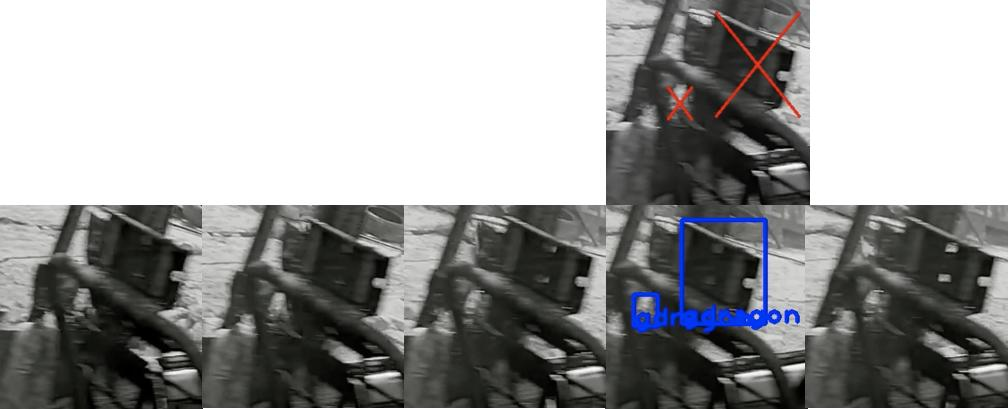
\includegraphics[width=\linewidth]{denoise.jpg}
\caption{Example of removal of bad bounding boxes. Initial frames and bounding boxes (top) and bounding box changes made by our algorithm (bottom). }
\label{figure:denoise}
\end{figure}

\begin{figure}[!t]
\centering
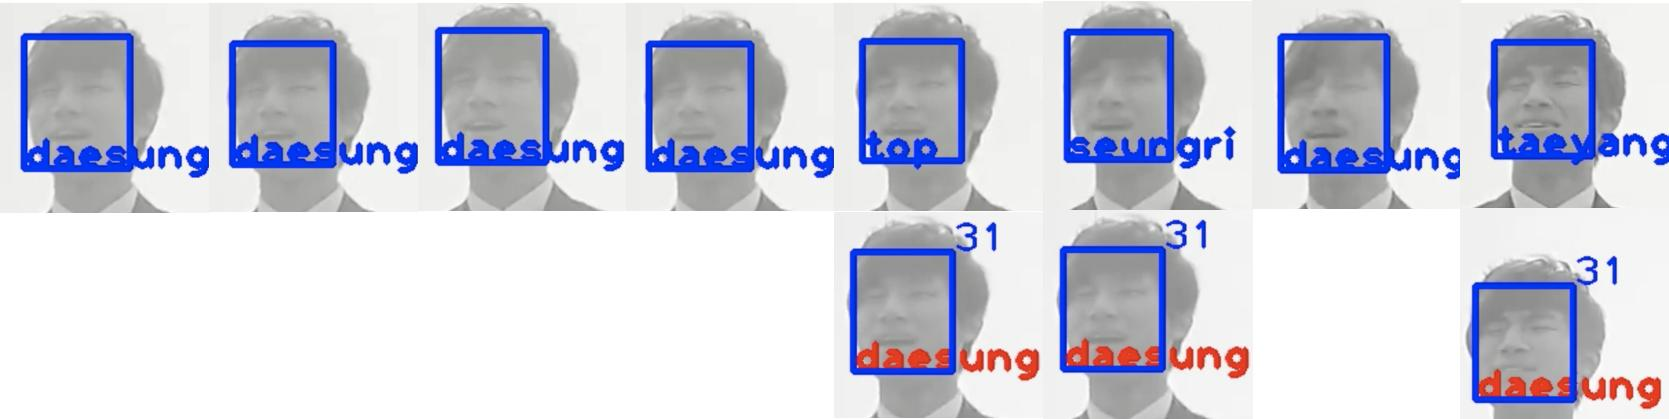
\includegraphics[width=\linewidth]{labels.jpg}
\caption{Example of label denoising. Initial frames and bounding boxes (top) and bounding box changes made by our algorithm (bottom). }
\label{figure:labels}
\end{figure}

\begin{figure}[!t]
\centering
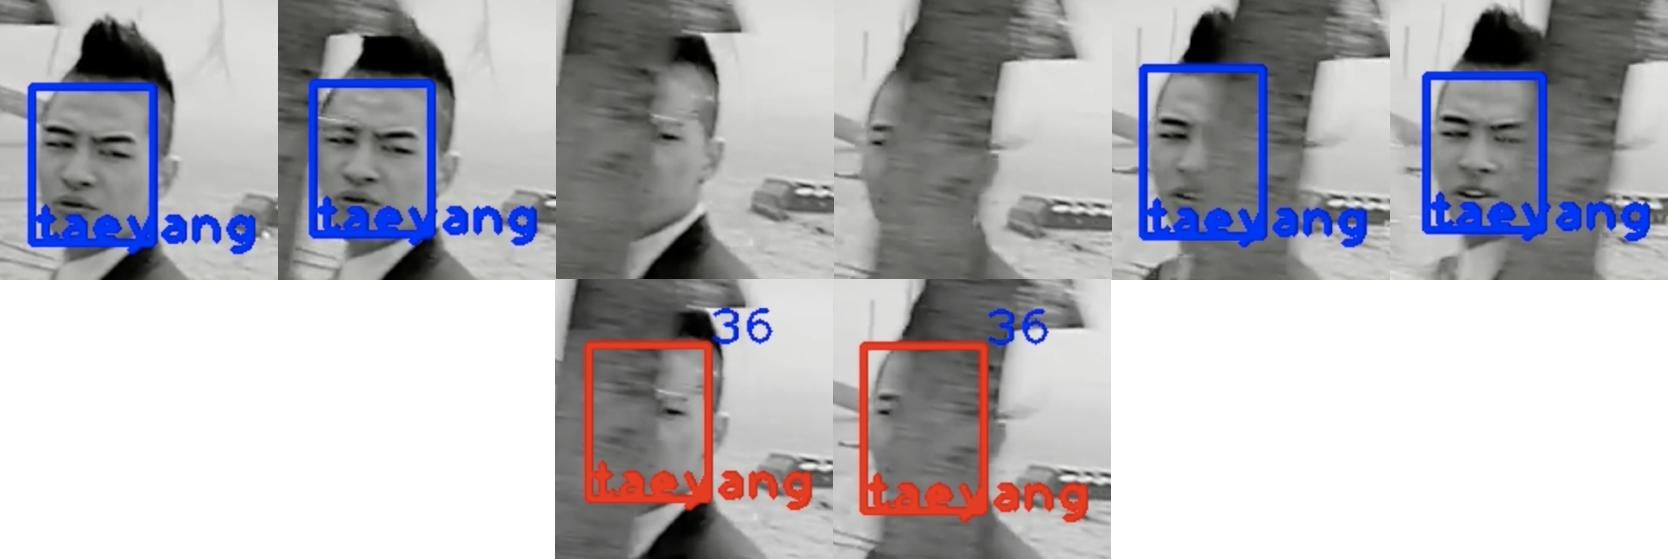
\includegraphics[width=\linewidth]{linear-interpolation.jpg}
\caption{Example of linear interpolation of missing bounding boxes. Initial frames and bounding boxes (top) and bounding box changes made by our algorithm (bottom). }
\label{figure:linear-interpolation}
\end{figure}

Numerically, we found that 93\% of the clusters were correctly labeled, 6\% of the final bounding boxes were added in by our algorithm (linear interpolation), and 29\% of the final bounding boxes have
labels which were either corrected or inferred by our algorithm. More complete results and the full videos can be found at the project's Github page \footnote{\url{https://github.com/ttv2107/UML-project}}.

\section{Conclusion}
We have given a simple and efficient algorithm for post-processing the output of running frame by frame detection and recognition algorithms on videos. Our algorithm makes
relatively limited assumptions on the inter frame structure when compared to tracking algorithms. This allows our algorithm to robustly handle frame switches, long occlusions, and
target objects coming in and out of the video. Additionally, by exploiting the video structure we are able to get very clean labels and bounding boxes, much cleaner than what is
returned directly by the
detection/recognition algorithms.

In future work, various directions could be explored to improve this algorithm. Most notably the third and fourth steps could be improved. For the merging of similar clusters it would be good
to develop more technical and robust ways of doing this. Techniques of hierarchical clustering or running DBSCAN with various different sets of parameters could be explored. For the fourth step,
better models could be devised than the linear one. Some sort of particle motion model which would take into account velocity could give better results. Alternatively, looking at detection confidence in
regions selected by the linear or alternative motion models could help locate the face more accurately. Finally, replacing MTCNN with an online detection/recognition algorithm could allow for interesting
modifications to our algorithm with the goal of making it work online.

\subsubsection*{Acknowledgments}

We thank Professor Verma as well as the TAs and students of the Fall 2018 Topics in Unsupervised Learning class for having provided us the opportunity
and the ideas necessary in the creation of this work.

\newpage
\bibliographystyle{unsrt}
\bibliography{final_report}

\end{document}
